\subchapter{Getting started}{Learn how to interact with
the board and how to reflash it}

\section{Board access through the serial line}

The first thing you need when working with a board is to access one of
the serial ports of the processor.

On the Microchip board, the processor's \code{DBGU} port can be accessed
through the \code{J14} connector.

\begin{center}
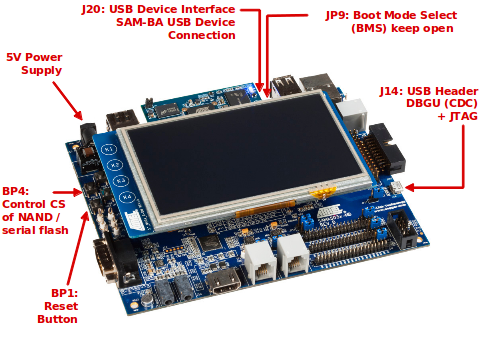
\includegraphics[width=8cm]{labs/boottime-getting-started/a5d3x_board_presentation.png}
\\
SAMA5D3x EK board connectors \\
{\small
(Source:
\url{http://www.at91.com/linux4sam/bin/view/Linux4SAM/GettingStarted_a5d3x})}
\end{center}

Power on your board and take a USB to micro USB cable provided by your
instructor. Connect the micro USB end to \code{J14}, and the other end
to your PC.

You should now have a device file named \code{/dev/ttyACM0}:

\begin{verbatim}
$ ls -la /dev/ttyACM0
crw-rw---- 1 root dialout 166, 0 Jul  9 16:48 /dev/ttyACM0
\end{verbatim}

You will use this device file to access the serial connection to the board.
As you can see, Ubuntu only allows the \code{root} user and
\code{dialout} group to access this file. A solution is to add your user
to this \code{dialout} group:

\begin{verbatim}
sudo adduser $USER dialout
\end{verbatim}

{\bf Important}: for the group change to be effective, in Ubuntu 18.04, you have to
{\em completely reboot} the system \footnote{As explained on
\url{https://askubuntu.com/questions/1045993/after-adding-a-group-logoutlogin-is-not-enough-in-18-04/}.}.
A workaround is to run \code{newgrp dialout}, but it is not global.
You have to run it in each terminal.

To communicate with the board through the serial port, install a
serial communication program, such as \code{picocom}\footnote{
\code{picocom} is one of the simplest utilities to access a
serial console. It works in a simple terminal. \code{minicom} has more
features, but is also more complex to configure.}:

\begin{verbatim}
sudo apt install picocom
\end{verbatim}

Now, run the below command, to start serial communication on
\code{/dev/ttyACM0}, with a baudrate of 115200:

\begin{verbatim}
$ picocom -b 115200 /dev/ttyACM0
picocom v1.4

port is        : /dev/ttyACM0
flowcontrol    : none
baudrate is    : 115200
parity is      : none
databits are   : 8
escape is      : C-a
noinit is      : no
noreset is     : no
nolock is      : no
send_cmd is    : ascii_xfr -s -v -l10
receive_cmd is : rz -vv

Terminal ready
\end{verbatim}

If you wish to exit \code{picocom}, press \code{[Ctrl][a]} followed by
\code{[Ctrl][x]}.

\section{Flash the board}

First, create the working directory for this lab:

\begin{verbatim}
mkdir /opt/boot-time-labs/flashing
cd /opt/boot-time-labs/flashing
\end{verbatim}

It is now time to flash the board with the filesystem used in this
workshop. To do so, we will use a tool named SAM-BA, provided by
ATMEL. You can download SAM-BA at
\url{http://atmel.com/Images/sam-ba_2.12.zip}, or take it from the USB
flash drive as follows:

\begin{verbatim}
cp /media/$USER/BootTime/downloads/sam-ba_2.12.zip .
unzip sam-ba_2.12.zip
\end{verbatim}

Now add the SAM-BA directory to your \code{PATH} environment variable
by adding the below line at the end of your \code{~/.bashrc} file:
\begin{verbatim}
export PATH=$PATH:/opt/boot-time-labs/flashing/sam-ba_cdc_cdc_linux/
\end{verbatim}

Now, source your \code{.bashrc} to load the new definition in your
current terminal:
\begin{verbatim}
source ~/.bashrc
\end{verbatim}

We will use the Buildroot demo from Linux4SAM\footnote{The original demo
was found on
\url{ftp://at91.com/pub/demo/linux4sam_4.0/linux4sam-buildroot-sama5d3xek_linux4sam_4.0.zip},
but it may have changed since the time we prepared these instructions.
Using the original copy is a way to make sure that the instructions are
not broken by Microchip updates.}.

Let's take the copy of the demo from the USB flash drive and extract it:

\begin{verbatim}
cp /media/$USER/BootTime/downloads/sama5d3xek-demo.tar.xz .
tar xf sama5d3xek-demo.tar.xz
\end{verbatim}

SAM-BA requires an extra Ubuntu package:

\begin{verbatim}
sudo apt install libxss1
\end{verbatim}

If you have a 64 bit system (if the \code{arch} command returns
\code{x86_64}, SAM-BA also needs the 32-bit libraries:

\begin{verbatim}
sudo apt install ia32-libs
\end{verbatim}

Make sure that \code{JP9} is open to enable booting from the
on-chip boot ROM.

To be able to flash the board, you have to stop the CPU in RomBOOT
mode. While in this mode, you will be able to use SAM-BA to
communicate directly with the CPU. To enter the RomBOOT mode, you have to
press and hold \code{PB4} while resetting the board using \code{PB1}.
\code{RomBOOT} should appear on your serial console and the board will
stop there.

If provided by the instructor, take a second USB to micro USB cable.
If you only have one such cable, exit \code{picocom} and disconnect
the one you were using for the serial console, for the time of the
flashing operation.

Connect your cable to \code{J20}, the SAM-BA interface. A device named
\code{/dev/ttyACM1} (or \code{/dev/ttyACM0} if you disconnected the
serial line) should then appear on your system:

\begin{verbatim}
$ ls -la /dev/ttyACM1
crw-rw---- 1 root dialout 166, 1 Jul  9 16:48 /dev/ttyACM1
\end{verbatim}

You are now ready to flash the board using SAM-BA.

\begin{verbatim}
cd sama5d3xek-demo/
sam-ba /dev/ttyACM1 AT91SAMa5d3x-EK sama5d3xek_demo_linux_nandflash.tcl
\end{verbatim}

If everything went smoothly, you should see the \code{DONE} keyword
after a few minutes in your terminal:

\begin{verbatim}
...
-I- Complete 99%
-I- 	Writing: 0x20000 bytes at 0x2420000 (buffer addr : 0x2001052C)
-I- 	0x20000 bytes written by applet
-I- === DONE. ===
\end{verbatim}

If you are facing trouble or just need more details about how to use and
flash the Microchip board, or if you wish to run the same steps from
Windows, you should read the
\url{http://www.at91.com/linux4sam/bin/view/Linux4SAM/GettingStarted_a5d3x}
page.

Now, remove the USB cable used for SAM-BA. If you have only one cable,
connect it again to the serial line and start \code{picocom} again.
Then, reset your board with \code{PB1}.

In the serial console, you will see your device boot. The first boot
will be slow, because of the time needed to generate an SSH key pair.
After a few minutes at most, the board will start showing a video on
its LCD.
